\documentclass[a4paper, 12pt]{article}
\usepackage[utf8x]{inputenc}
\usepackage{cmap}
\usepackage[english, russian]{babel}
\usepackage{indentfirst}
\usepackage[left=20mm, top=20mm, right=20mm, bottom=20mm]{geometry}
\usepackage{tikz}
\usepackage{float}
\usepackage{amsmath, amsfonts, amssymb}
\usepackage{graphicx}
\usepackage{fancybox, fancyhdr}
\usepackage{hyperref}
\usepackage{listings}
\usepackage{caption}
\usepackage{subcaption}
\usepackage{xcolor}
\pagestyle{fancy}
\fancyhf{}
\fancyhead[L]{Лабораторная работа №6}
\fancyhead[R]{Частотные методы}
\fancyfoot[C]{\thepage}
\graphicspath{{images/}}
\usetikzlibrary{patterns}
\definecolor{LightGray}{gray}{0.95}
\definecolor{LightGray2}{gray}{0.7}
\lstdefinestyle{code}{
    language=Python,
    basicstyle=\footnotesize\ttfamily,
    % numbers=left,
    % numberstyle=\scriptsize\color{gray},
    % stepnumber=1,
    % numbersep=5pt,
    backgroundcolor=\color{LightGray},
    showspaces=false,
    showstringspaces=false,
    showtabs=false,
    tabsize=4,
    captionpos=b,
    breaklines=true,
    breakatwhitespace=false,
    frame=single,
    rulecolor=\color{LightGray2},
    linewidth=\linewidth,
    keywordstyle=\color{blue}\bfseries,
    commentstyle=\color{green!40!black},
    stringstyle=\color{purple},
    escapeinside={\%*}{*)},
    inputencoding=utf8x,
    xleftmargin=0pt,
    framexleftmargin=0pt,
    framexrightmargin=0pt
}
\lstset{style=code}
\hypersetup{
    colorlinks=true,
    linkcolor=blue,
    filecolor=magenta,
    urlcolor=cyan,
    pdftitle={contents setup},
    pdfpagemode=FullScreen,
}
\setlength{\parskip}{1.5mm}
\setlength{\headheight}{15pt}
\setlength{\footskip}{15pt}
\allowdisplaybreaks
\DeclareMathOperator{\sinc}{sinc}
\newcommand{\frc}[2]{\raisebox{2pt}{$#1$}\big/\raisebox{-3pt}{$#2$}}

\begin{document}
    \begin{titlepage}

        \begin{center}
        
\includegraphics[width=0.3\textwidth]{itmo.png} % requires itmo.png in /images folder
        \vfill

        Федеральное государственное автономное образовательное учреждение высшего образования
        «Национальный Исследовательский Университет ИТМО»\\

        \vfill
        {\large\bf ЛАБОРАТОРНАЯ РАБОТА №6}\\
        {\large\bf ПРЕДМЕТ «ЧАСТОТНЫЕ МЕТОДЫ»}\\
        {\large\bf ТЕМА «ОБРАБОТКА ИЗОБРАЖЕНИЙ»}
        \vfill

        \begin{flushright}
            \begin{minipage}{.45\textwidth}
            {
                \hbox{Лектор: Перегудин А. А.}
                \hbox{Практик: Пашенко А. В.}
                \hbox{Студент: Румянцев А. А.}
                \hbox{Поток: ЧАСТ.МЕТ. 1.3}
                \hbox{}
                \hbox{Факультет: СУиР}
                \hbox{Группа: R3241}
            }
            \end{minipage}
        \end{flushright}

        \vfill

        Санкт-Петербург\\
        2024
        \end{center}
    \end{titlepage}

    \tableofcontents

    \newpage
    \section{Задание 1. Фильтрация изображений с периодичностью}
    Скачаем изображение под номером 4 с данного \href{https://drive.google.com/drive/folders/1oewu85taKvyxAUhXNH48ImTFtI1SpFag}{гугл-диска}.
    \begin{figure}[H]
        \centering
        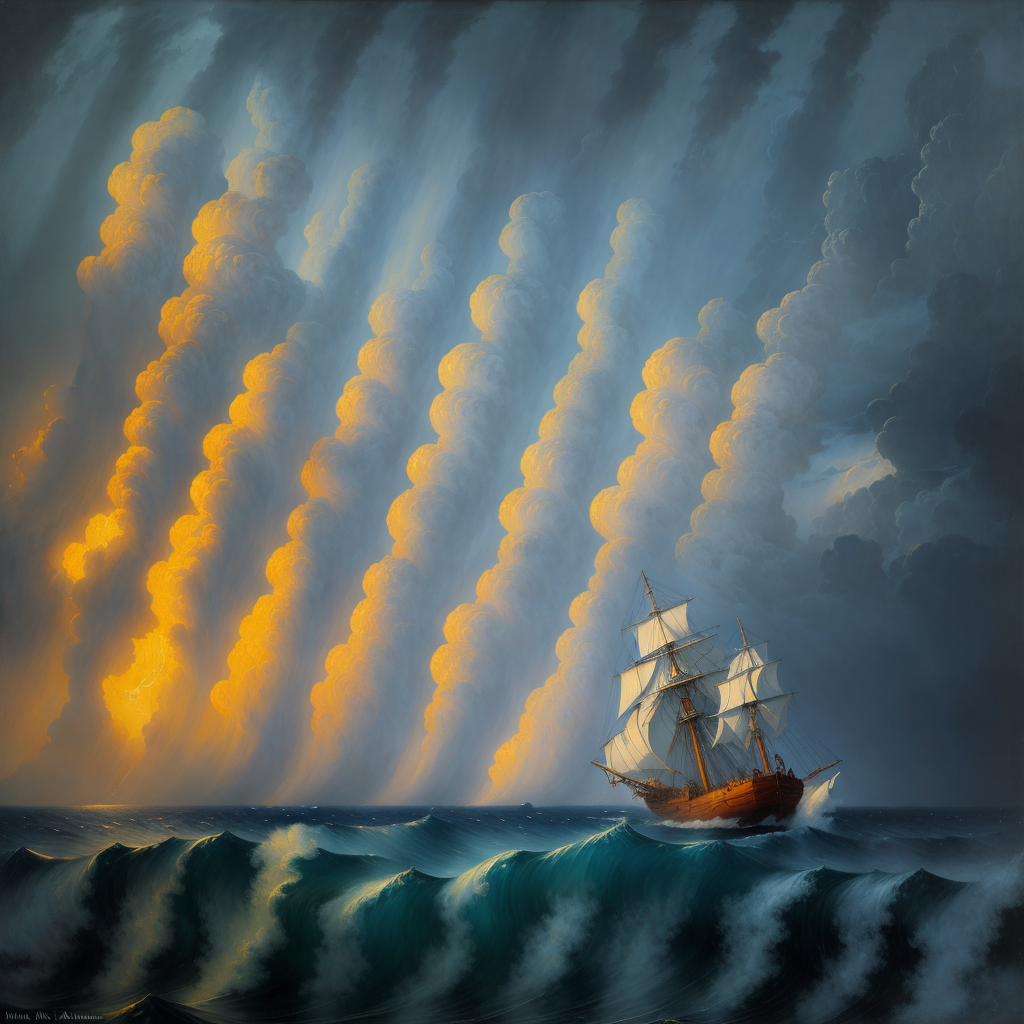
\includegraphics[width=0.45\linewidth]{4.png}
        \captionsetup{skip=0pt}
        \caption{Изображение, выбранное с представленного гугл-диска}
        \label{fig:4dotpng}
    \end{figure}


    Далее проделаем следующие шаги:
    \begin{enumerate}
        \item Загрузим это изображение в \texttt{python} с помощью библиотеки \texttt{pillow}.
        \item Преобразуем полученный массив к вещественному типу с помощью инструментов библиотеки \texttt{numpy}.
        Поделим все значения на 255 -- максимальное значение яркости цвета.
        \item Найдем двумерный Фурье-образ массива и сдвинем его в центр с помощью команд \texttt{fftshift(fft2(my\_image))}.
        Так как изображение цветное, выполним преобразование для каждого из цветовых каналов по отдельности.
        \item Разделим полученные образы каждого канала на массивы модулей и аргументов с помощью функций библиотеки \texttt{numpy} \texttt{abs} и \texttt{angle}.
        \item Для удобства работы, найдем логарифм от каждого массива модулей и нормализуем его
        значения в диапазон от 0 до 1. Чтобы избежать неопределённости в логарифме,
        предварительно прибавим ко всем значениям 1. Для этого понадобится команда \texttt{np.log1p()}. Для обратной операции \texttt{np.expm1()}.
        \item Объединим преобразованные каналы. Сохраним полученный массив (нормализованный логарифм модуля Фурье-образа)
        как изображение командой \texttt{save}, вызываемой от объекта \texttt{Image}.
        \item Проанализируем полученное на предыдущем шаге изображение. Найдем пики,
        соответствующие периодичности на исходной картинке.
        \item В программе редактирования изображений исправим полученный Фурье-образ: сгладим все ненужные цветовые пики, отвечающие за
        гармоники, от которых мы хотим избавиться.
        \item Восстановим картинку из отредактированного образа, проделав обратные шаги.  
    \end{enumerate}
    

    Цветной нормализованный логарифм модуля Фурье-образа данного изображения представлен на следующем
    рисунке.
    \begin{figure}[H]
        \centering
        \begin{subfigure}{0.45\textwidth}
            \centering
            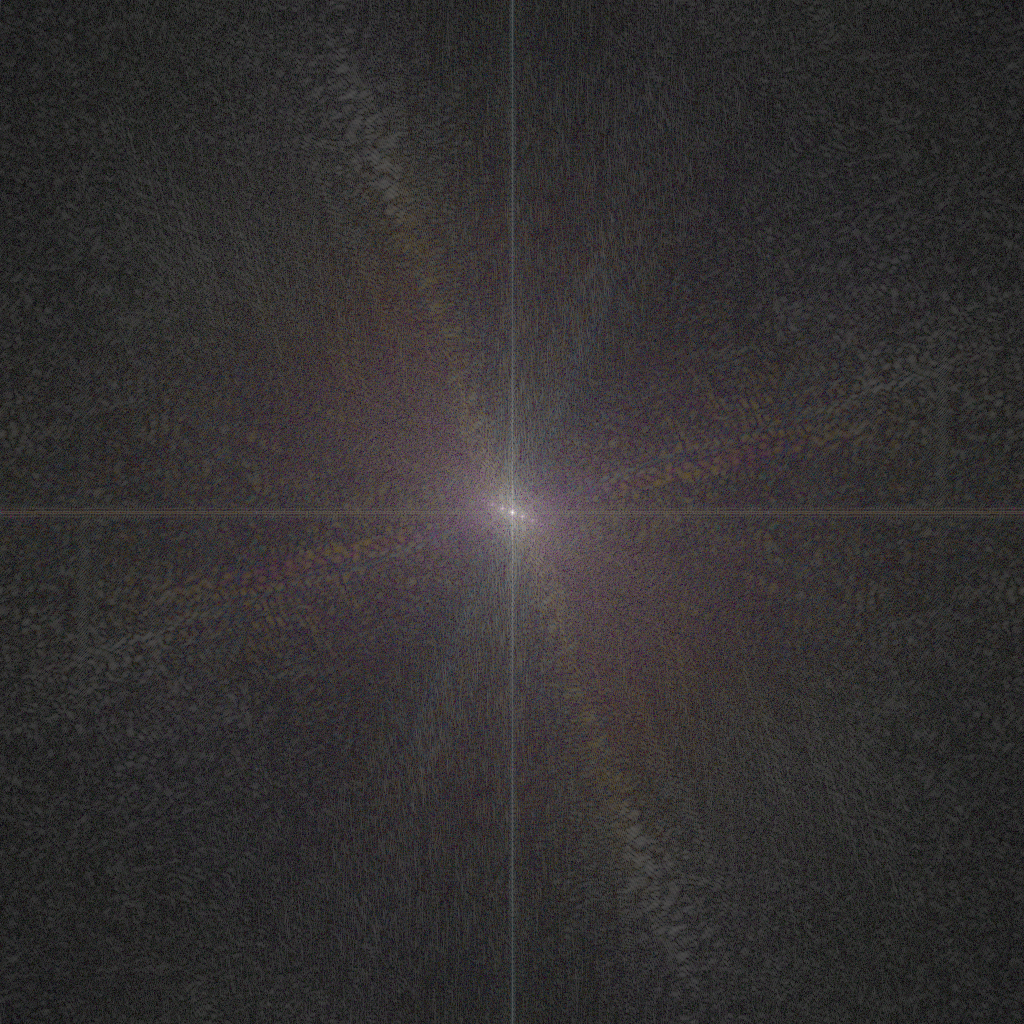
\includegraphics[width=\linewidth]{fft2.png}
            \caption{Цветной Фурье-образ изображения 4}
            \label{fig:4fft2}
        \end{subfigure}
        \begin{subfigure}{0.45\textwidth}
            \centering
            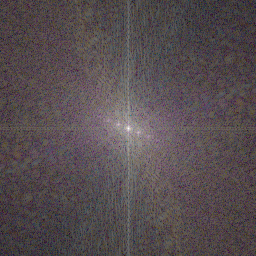
\includegraphics[width=\linewidth]{fft2_close.png}
            \caption{Приближение к центру Фурье-образа}
            \label{fig:4fft2cl}
        \end{subfigure}
        \caption{Нормализованный логарифм модуля Фурье-образа}
        \label{fig:fft2s}
    \end{figure}


    Видим на рис. \ref{fig:4fft2cl} около центра цветовые пики во второй и четвертой четвертях системы координат,
    если задать ее в центре изображения. Нам необходимо сгладить эти цветовые пики, отвечающие за синусоидальный шум
    на картинке. Сделаем это в редакторе изображений \texttt{paint} -- наложим <<пластыри>> из наиболее близких к пикам
    незасветленных областей с пикселями на места гармонического шума. Результат исправления расположен ниже.
    \begin{figure}[H]
        \centering
        \begin{subfigure}{0.45\textwidth}
            \centering
            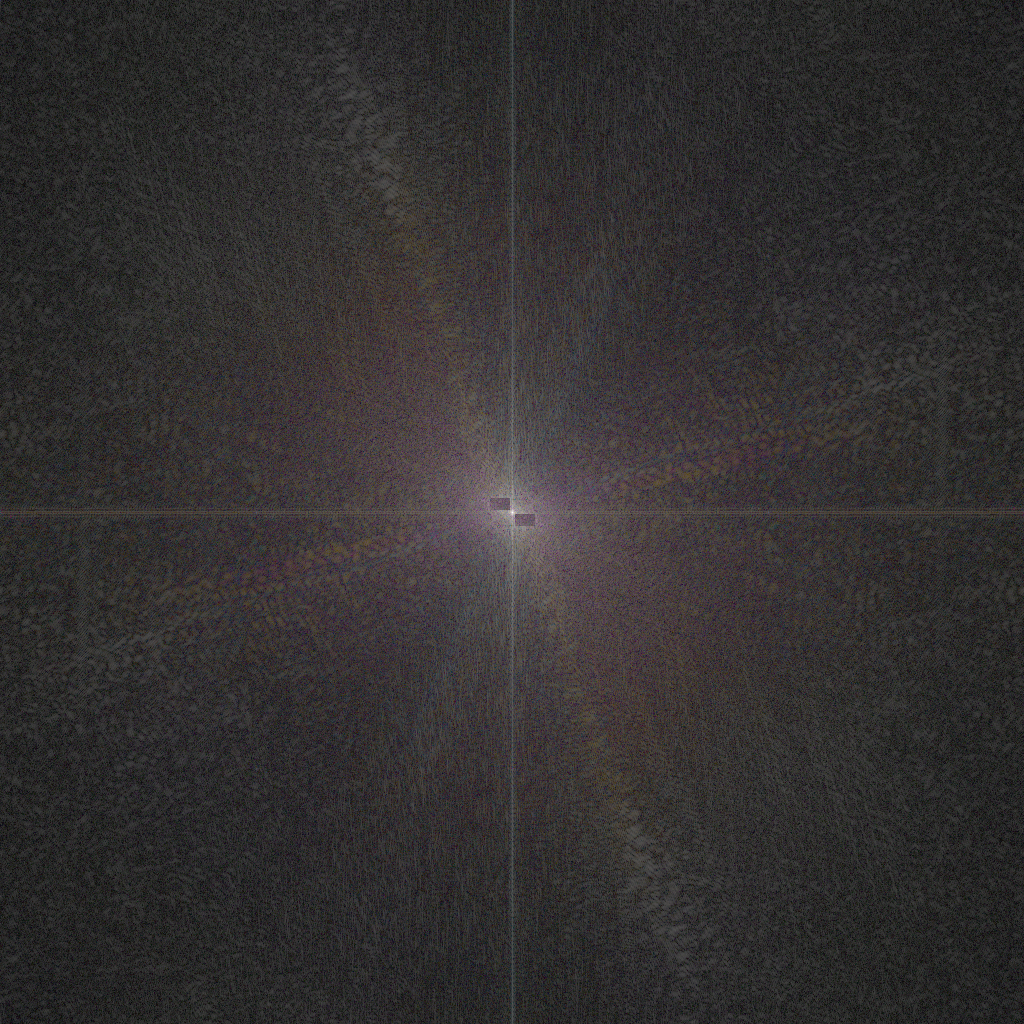
\includegraphics[width=\linewidth]{corr_fft2.png}
            \caption{Исправленный Фурье-образ изображения}
            \label{fig:corfft2}
        \end{subfigure}
        \begin{subfigure}{0.45\textwidth}
            \centering
            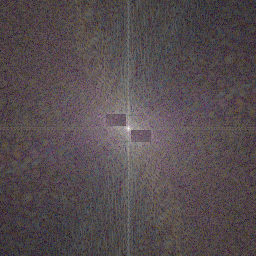
\includegraphics[width=\linewidth]{corr_fft2_close.png}
            \caption{Приближение к центру исправленного Фурье-образа}
            \label{fig:c4fft2cl}
        \end{subfigure}
        \caption{Исправленный нормализованный логарифм модуля Фурье-образа}
        \label{fig:cfft2s}
    \end{figure}


    Ниже представлен сравнительный рисунок -- оригинальное изображение и фильтрованное.
    Изображение без синусоидального шума (или с минимальным) выглядит более <<мягко>>.
    Море и небо стали более естественными.
    \begin{figure}[H]
        \centering
        \begin{subfigure}{0.45\textwidth}
            \centering
            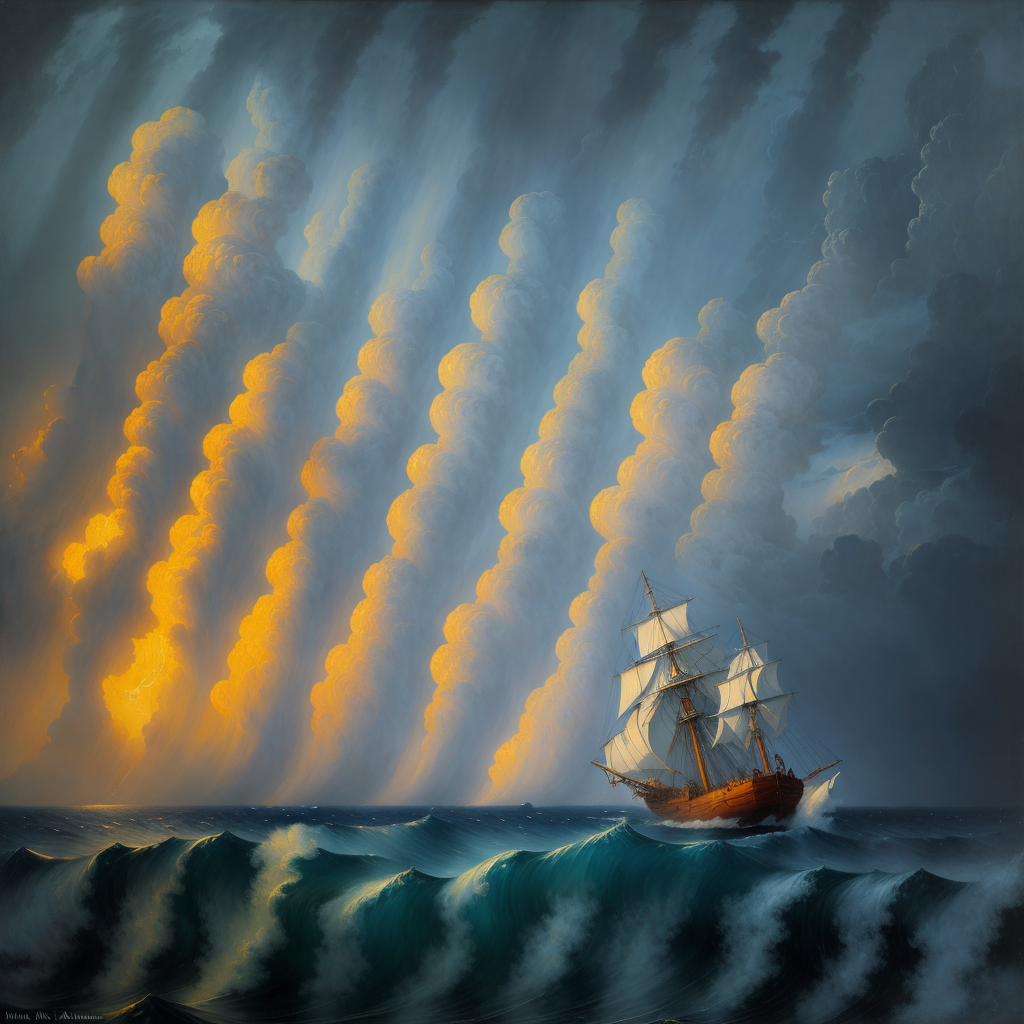
\includegraphics[width=\linewidth]{4.png}
            \caption{Исходное изображение}
            \label{fig:old}
        \end{subfigure}
        \begin{subfigure}{0.45\textwidth}
            \centering
            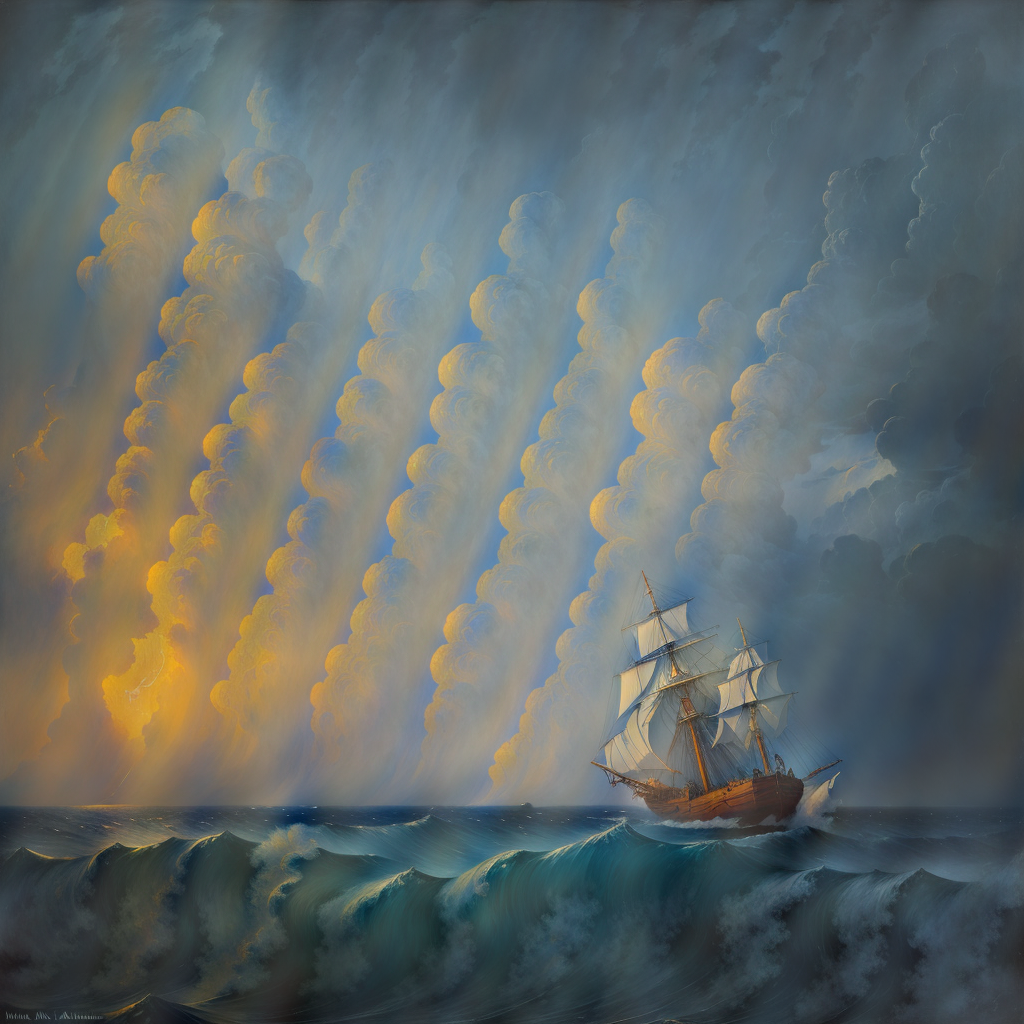
\includegraphics[width=\linewidth]{new4.png}
            \caption{Фильтрованное изображение}
            \label{fig:new}
        \end{subfigure}
        \caption{Сравнение исходного и фильтрованного изображений}
        \label{fig:oldnew}
    \end{figure}


    Для восстановления изображения понадобилась формула ниже:
    $$
    \hat{X}=|\hat{X}|_{new}\cdot e^{i\angle\hat{X}},
    $$
    где $\hat{X}$ -- Фурье-образ изображения, $|\hat{X}|_{new}$ фильтрованный массив модулей,
    $e^{i\angle\hat{X}}$ комплексное число с аргументом $\angle\hat{X}$, представляющим массив углов
    Фурье-образа. $|\hat{X}|_{new}$ отвечает за новые амплитуды частотных компонент, а $e^{i\angle\hat{X}}$
    за фазы исходных амплитуд. Без массива углов мы бы не смогли привести изображение к изначальной <<структуре>>.


    \subsection{Листинг для задания 1}
    Для реализации программ, необходимых для выполнения задания 1, были использованы язык программирования
    \texttt{python} с библиотеками \texttt{pillow} и \texttt{numpy}.
    \begin{lstlisting}[label=task1, caption={Программные методы, необходимые для задания 1}]
    from PIL import Image
    import numpy as np

    # Method to read image along the specified path
    def read_img(path: str):
        return Image.open(path)

    # Method to save image along the specified path
    def save_img(img: Image, path: str):
        img.save(path)

    # Method to convert an array to an image
    def convert_arr_to_img(arr):
        return Image.fromarray(arr)

    # Method to normalize data (ex. logarithm of abs(image))
    # Returns min and max to inverse the normalization
    def normalize(data):
        min_ = np.min(data)
        max_ = np.max(data)
        nz = (data - min_) / (max_ - min_)
        return nz, min_, max_
    
    # Method to remove normalization from data
    # Requires min and max to inverse normalization
    def denormalize(nz, min_, max_):
        return nz * (max_ - min_) + min_
    
    # Method to split rgb image array into 3 channels
    def rgb_channels(img: Image):
        img_arr = np.array(img)
        r = img_arr[:, :, 0]
        g = img_arr[:, :, 1]
        b = img_arr[:, :, 2]
        return r, g, b
    
    # Method to split rgb image angles array into 3 for each channel
    def rgb_angles(angles):
        ar = angles[:, :, 0]
        ag = angles[:, :, 1]
        ab = angles[:, :, 2]
        return ar, ag, ab

    # Method to apply fft2 to a channel
    # Uses special algorithm for convenience
    def fft2_channel(channel):
        channel = channel.astype(np.float64) / 255
        fft_ = np.fft.fftshift(np.fft.fft2(channel))
        abs_ = np.abs(fft_)
        angle = np.angle(fft_)
        log = np.log1p(abs_)
        nz, min_, max_ = normalize(log)
        return nz, min_, max_, angle
    
    # Method to apply ifft2 to a channel
    # Inverts all the steps of the special algorithm
    def ifft2_channel(channel, angle, min_, max_):
        channel = channel.astype(np.float64) / 255
        denor = denormalize(channel, min_, max_)
        abs_ = np.expm1(denor)
        col_res = abs_ * np.exp(1j * angle)
        ifft_ = np.fft.ifft2(np.fft.ifftshift(col_res))
        return np.real(ifft_)
    
    # Method to apply fft2 to an image. Processes three channels at once
    def fft2(img: Image):
        r, g, b = rgb_channels(img)
    
        nzr, min_r, max_r, ar = fft2_channel(r)
        nzg, min_g, max_g, ag = fft2_channel(g)
        nzb, min_b, max_b, ab = fft2_channel(b)
    
        res = np.stack((nzr, nzg, nzb), axis=2)
        res = (res * 255).astype(np.uint8)
    
        ang = np.stack((ar, ag, ab), axis=2)
        nz_min_max = [(min_r, max_r), (min_g, max_g), (min_b, max_b)]
        return res, ang, nz_min_max
    
    # Method to apply ifft2 to an image. Processes three channels at once
    def ifft2(img: Image, angles, nz_min_max):
        r, g, b = rgb_channels(img)
        ar, ag, ab = rgb_angles(angles)
    
        nz_r_min, nz_r_max = nz_min_max[0][0], nz_min_max[0][1]
        nz_g_min, nz_g_max = nz_min_max[1][0], nz_min_max[1][1]
        nz_b_min, nz_b_max = nz_min_max[2][0], nz_min_max[2][1]
    
        new_r = ifft2_channel(r, ar, nz_r_min, nz_r_max)
        new_g = ifft2_channel(g, ag, nz_g_min, nz_g_max)
        new_b = ifft2_channel(b, ab, nz_b_min, nz_b_max)
    
        res = np.stack((new_r, new_g, new_b), axis=2)
        res = normalize(res)[0] * 255
        return res.astype(np.uint8)

    # Helper method for external use of fft2
    def fft2_2img(img: Image):
        res, ang, nz_min_max = fft2(img)
        return convert_arr_to_img(res), ang, nz_min_max
    
    # Helper method for external use of ifft2
    def ifft2_2img(img: Image, angles, nz_min_max):
        return convert_arr_to_img(ifft2(img, angles, nz_min_max))
    \end{lstlisting}


    Все вышеперечисленные наработки используются в программе, представленной ниже.
    \begin{lstlisting}[label=task11, caption={Реализация задания 1}]
    import img_utils as iu

    # Specify the image source
    src = 'fm_lab6/src'
    img_path = f'{src}/4.png'

    # Specify where to render the result
    render_to = 'fm_lab6/renders/task1'
    rimg_path = f'{render_to}/fft2.png'
    reimg_path = f'{render_to}/new4.png'

    # Specify the corrected image source
    # Parameter "corrected" if that source does exist
    corr_im_path = f'{src}/corr_fft2.png'
    corrected = True

    # Reading image, applying fft2 and saving the result
    img = iu.read_img(img_path)
    ans, ang, nzmm = iu.fft2_2img(img)
    iu.save_img(ans, rimg_path)

    # Reading corr. im., applying ifft2 to recover im. and saving the res.
    if corrected:
        img2 = iu.read_img(corr_im_path)
        ans2 = iu.ifft2_2img(img2, ang, nzmm)
        iu.save_img(ans2, reimg_path)
    \end{lstlisting}


    \section{Задание 2. Размытие изображения}
\end{document}